\section{L'idée d'une électronique moléculaire}
\footnote{Cet état de l'art se base sur ceux présentés dans \cite{3} et \cite{4}}C'est en 1974 que l'idée d'utiliser des molécules uniques dans la fabrication de composants électroniques est apparue, lors d'un séminaire tenu par Arieh Aviram et Mark Ratner.

Cette date peut être considérée comme la naissance de ce que l'on appelle l'électronique moléculaire.
Le but étant à la fois de permettre d'aller encore plus loin dans la miniaturisation des composants en microélectronique mais aussi d'adopter une technique de fabrication basée sur l'auto-organisation de petites molécules en structure complexe: technique dite “bottom-up”.
\section{Le premier transistor moléculaire}
Mais en 1974, on est encore loin de l'utilisation concrète de molécules uniques dans l'électronique, et il faudra attendre 1995 pour que la première mesure de courant à travers une molécule unique soit réalisée à l'aide d'un microscope à effet tunnel (STM).

De nombreuses autres expériences vont suivre, et en 1997 apparaît la technique de “break junction” qui consiste à effectuer la cassure d'un pont métallique sur substrat flexible en pliant le substrat. On peut alors sans STM mesurer les caractéristiques de molécules uniques, et caractériser l'influence de la taille du gap. Mais on n'a toujours pas de grille pour pouvoir permettre l'utilisation comme transistor.

Ce n'est qu'en 2000 que J.W. Park et son équipe utiliseront une technique d'électromigration\footnote{Nous présentons plus en détail l'électromigration dans une partie dédiée.} pour permettre la fabrication du premier transistor à molécule unique avec une molécule de fullerène C$_{60}$. D'autres groupes vont alors utiliser cette même technique en utilisant d'autres molécules et leurs propriétés, et en particulier des aimants moléculaires (SMM) pour leurs propriétés liées au spin. Mais aussi en mettant en place des expériences qui permettront d'effectuer les mesures à quelques milliKelvins.

\section{De nouvelles molécules: vers la spintronique moléculaire}
En 2006 l'utilisation de SMM débute afin de permettre la réalisation de dispositifs de spintronique moléculaire. Les équipe de H.S.J Van der Sant (à Cornell) et D.C. Ralph (à Delft) vont étudier tout d'abord l'aimant moléculaire le plus fameux, Mn$_{12}$, mais les résultats sont peu satisfaisants et la première réalisation d'un véritable dispositif de spintronique moléculaire est réalisé à Delft par l'équipe de Ralph en 2008 à l'aide d'une molécule de N@C$_{60}$ (atome d'azote piégé dans une molécule de fullerène). Il est possible avec une telle molécule de retrouver dans les mesures de transport ses propriétés magnétiques.\\

\begin{figure}[h]
    \begin{center}
        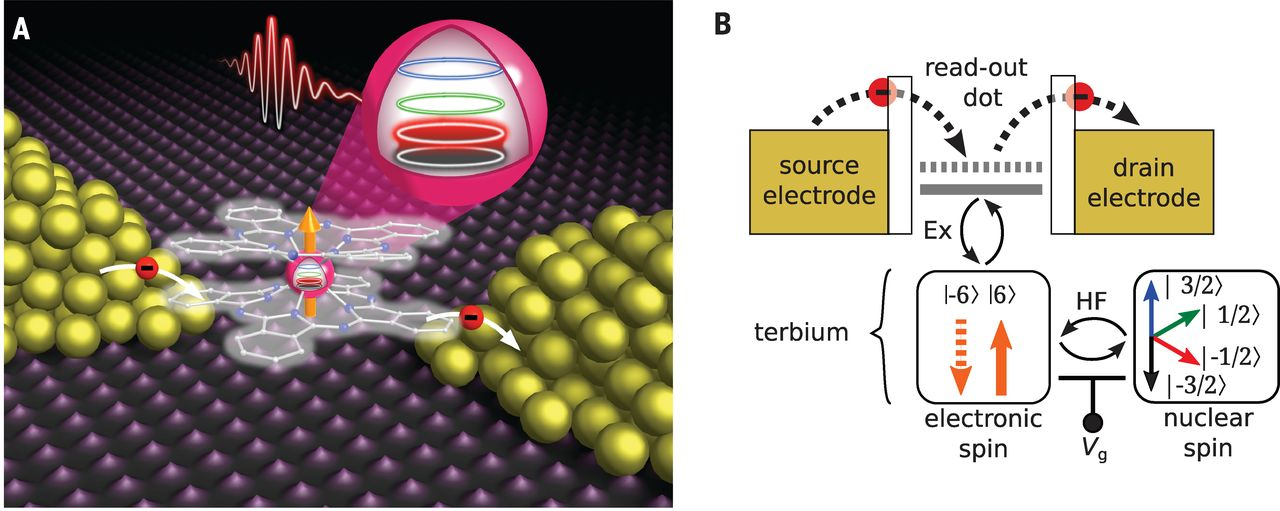
\includegraphics{Images/TbPc2.jpg}
        \caption{Vue de la molécule de TbPc$_2$, et schéma de principe.}
        \label{fig:}
    \end{center}
\end{figure}

Cependant cette molécule n'est pas un aimant moléculaire, et il est donc impossible de se servir des propriétés quantiques liées au magnétisme moléculaire. Les équipes vont alors se tourner vers d'autres aimants moléculaires notamment Fe$_{4}$ (à Delft), Ni$_{4}$(à Cornell)...etc et la molécule TbPc$_{2}$ (molécule organique avec un atome de Terbium) à l'institut Louis Néel dans l'équipe de Franck Balestro. L'aimant moléculaire TbPc$_{2}$ utilisé dans un transistor à molécule unique a permis de réaliser la lecture électrique et la manipulation quantique d'un spin nucléaire unique.
